\documentclass[utf8,12pt]{beamer}

\usepackage{graphicx}
\usepackage{amsmath}
\usepackage{bm} % bold math symbols
\usepackage{tgpagella} % Gyre pagella -- based on palatino
\usepackage[english]{babel}
\usepackage[binary-units]{siunitx}
\usepackage[absolute,overlay]{textpos}
\usepackage{verbatim}

\usetheme{default}
\usecolortheme{seagull}
\usefonttheme{serif}
\setbeamertemplate{navigation symbols}{}
\logo{\includegraphics[height=1.5cm]{img/robot.pdf}}

\input{math-defs.tex}

\title{Exploiting GPS in Monte Carlo Localization}
\author{Jakub Marek}


\newcommand{\imageframe}[3]{{
\setbeamertemplate{background}{
    \vbox to \paperheight{\vfil\hbox to \paperwidth{\hfil
    \includegraphics[width=\paperwidth,height=\paperheight,keepaspectratio]{#1} %%% nodep
    \hfil}\vfil}
    }
\setbeamercolor{background canvas}{bg=#2}
\begin{frame}[plain]
\end{frame}
}}


\begin{document}


\begin{frame}[plain]
    \titlepage
\end{frame}

\begin{frame}{Main Idea}
    \begin{itemize}
        \item Outdoor robots need position information
        \item Improve precision available from GPS
        \begin{itemize}
            \item Individual measurements
            \item Combination with other sensors
        \end{itemize}
        \item Improve error characterization
        \item Explore inner workings of GPS
    \end{itemize}
\end{frame}

%%%% dependency img/01.jpg
%\imageframe{img/01.jpg}{black}

\begin{frame}{Why GPS}
    \begin{textblock*}{3cm}[1,1](115mm,45mm)
        \includegraphics[height=3cm]{img/receiver.jpg}
    \end{textblock*}
    \begin{itemize}
        \item Worldwide absolute position
        \item No preparation required
        \item Cheap (?!)
    \end{itemize}

    \begin{itemize}
        \item Low precision from consumer GPS receivers
        \item Low measurement frequency
    \end{itemize}
\end{frame}

\begin{frame}{Why Monte Carlo Localization}
    \begin{itemize}
        \item Probabilistic localization algorithm
        \item Simple to understand and implement
        \begin{itemize}
            \item Simulate a swarm of possible robots
            \item Compare the actual and simulated sensor readings
        \end{itemize}
        \item Only requires probability of a measurement
        \item Arbitrary shapes of probability densities
    \end{itemize}

    \begin{itemize}
        \item More computationally intensive than Kalman Filter
    \end{itemize}
\end{frame}

\begin{frame}{GPS -- Basic Principles}
    \begin{itemize}
        \item Measuring time of flight of radio signals
        \begin{itemize}
            \item Ideally: position = intersection of spherical surfaces
            \item Reality: 4D conical surfaces (3D positions + time)
        \end{itemize}
    \vspace{0.5cm}
    \centerline{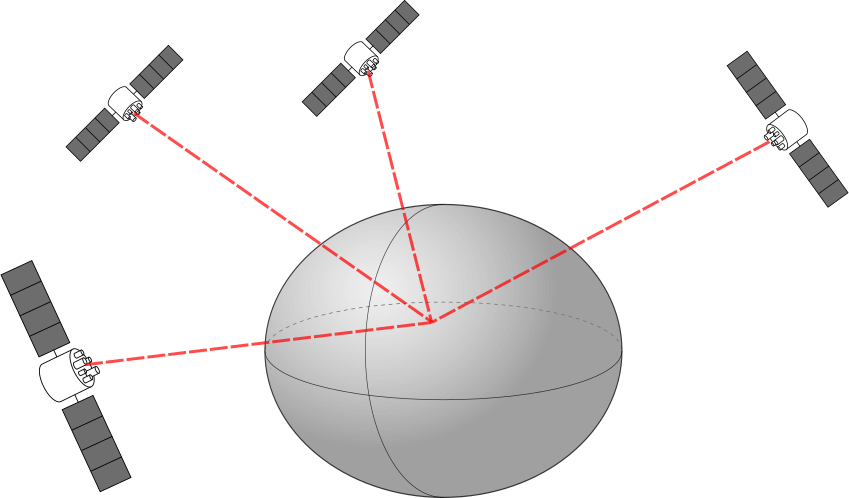
\includegraphics[height=5cm]{img/pseudoranges.pdf}}
    \end{itemize}
\end{frame}

\begin{frame}{GPS -- Basic Principles}
    \begin{itemize}
        \item Pseudorange
        \begin{itemize}
            %\item \(\rho = \speedoflight (\recrxtime - \svtxtime)\)
            \item Distance corresponding to time of flight
            \begin{itemize}
                \item Transmission time according to satellite clock
                \item Receipt time according to receiver clock
            \end{itemize}
        \end{itemize}
        \item Doppler measurements
        \begin{itemize}
            \item Relative velocities of satellite and receiver
        \end{itemize}
    \end{itemize}
\end{frame}

\begin{frame}[fragile]{GPS with MCL -- Simple Approach}
    \begin{itemize}
        \item Most GPS receivers provide NMEA output
        \begin{itemize}
            \item{\footnotesize\verb=$GPGSA,A,3,04,05,,09,12,,,24,,,,,2.5,1.3,2.1*39=}
            \item Contains WGS84 lat/lon/alt coordinates and HDOP
        \end{itemize}
        \item Can be used as a position input almost immediately
        \begin{itemize}
            %\item Rayleigh distribution, \( \sigma = \frac{\sqrt{(a \HDOP)^2 + b^2}}{\sqrt{2}} \)
            \item Horizontal position errors only
            \item No characterization of velocity error
        \end{itemize}
    \end{itemize}
\end{frame}

\begin{frame}[plain]{Error vs. HDOP}
\begin{center}
\centerline{\includegraphics[height=8cm]{generated/wgs84-hdop-error.pdf}}
\end{center}
\end{frame}

\begin{frame}{GPS with MCL -- Low Level Approach}
    \begin{itemize}
        \item Each pseudorange measurement as localization input
        \item Allows to use Doppler measurements
        \item Specific to a GPS chipset
        \begin{itemize}
            \item Data not in NMEA protocol
            \item SiRF III
        \end{itemize}
    \end{itemize}
\end{frame}

\begin{frame}{Low Level Approach}
    \begin{itemize}
        \item Need to consider atmospheric delays
        \begin{itemize}
            \item Estimating low frequency errors as a part of the robot's state
        \end{itemize}
        \item Approximately \SI{7}{\meter} \(1\sigma\) error for single measurement
        \begin{itemize}
            \item Similar precision to the simple NMEA data
            \item Room for improvement
        \end{itemize}
    \end{itemize}
\end{frame}

\begin{frame}[plain]{Pseudorange Errors}
\begin{center}
\centerline{\includegraphics[height=8cm]{generated/pseudorange-errors.pdf}}
\end{center}
\end{frame}

\begin{frame}{Pseudoranges vs. WGS84 Data}
    \begin{itemize}
        \item Error characterization
        \item Velocity measurements
        \item Possibility to further process measurements
        \begin{itemize}
            \item Multipath

        \end{itemize}
    \end{itemize}

    \begin{itemize}
        \item Computing power
        \item More intrusive in localization algorithm
    \end{itemize}
\end{frame}

\begin{frame}{Implementation}
    \begin{itemize}
        \item Tools for analyzing GPS errors
        \begin{itemize}
            \item Recording and off-line processing
        \end{itemize}
        \item SiRF III chip
        \item Number of implementation challenges
        \begin{itemize}
            \item Documentation
            \item Clock jumps
            \item Doppler measurements
            \item Uncovered error in velocity processing
        \end{itemize}
    \end{itemize}
\end{frame}

\begin{frame}[plain]{Velocity Error Histogram}
\begin{center}
\centerline{\includegraphics[height=8cm]{generated/velocity-histogram.pdf}}
\end{center}
\end{frame}

\begin{frame}{Conclusion}
    \begin{itemize}
        \item WGS84 data
        \begin{itemize}
            \item Realistic, simple to use
        \end{itemize}
        \item Low level approach
        \begin{itemize}
            \item More complex, more flexible
        \end{itemize}
        \item Overview of GPS and SiRF
        \item Framework for further experimenting
    \end{itemize}
\end{frame}

{
\setbeamercolor{background canvas}{bg=black}
\begin{frame}[plain]
\end{frame}
}

%\begin{frame}[plain]
%    \centerline{\Large Thank you}
%\end{frame}
%
%\begin{frame}[plain]
%    \centerline{\Large Questions?}
%\end{frame}

\end{document}
